% Copyright (C) 2020 Saurabh Joshi
%% 
\let\negmedspace\undefined
\let\negthickspace\undefined

\documentclass[journal,12pt,onecolumn]{IEEEtran}
%\documentclass[journal,12pt,twocolumn]{IEEEtran}
%
\usepackage{setspace}
\usepackage{gensymb}
%\doublespacing
\singlespacing

%\usepackage{graphicx}
%\usepackage{amssymb}
%\usepackage{relsize}
\usepackage[cmex10]{amsmath}
%\usepackage{amsthm}
%\interdisplaylinepenalty=2500
%\savesymbol{iint}
%\usepackage{txfonts}
%\restoresymbol{TXF}{iint}
%\usepackage{wasysym}
\usepackage{amsthm}
\usepackage{mathrsfs}
\usepackage{txfonts}
\usepackage{stfloats}
\usepackage{cite}
\usepackage{cases}
\usepackage{subfig}
%\usepackage{xtab}
\usepackage{longtable}
\usepackage{multirow}
%\usepackage{algorithm}
%\usepackage{algpseudocode}
\usepackage{enumitem}
\usepackage{mathtools}
\usepackage{tikz}
\usepackage{circuitikz}
\usepackage{verbatim}
\usepackage{hyperref}
%\usepackage{stmaryrd}
\usepackage{tkz-euclide} % loads  TikZ and tkz-base
%\usetkzobj{all}
\usepackage{listings}
    \usepackage{color}                                            %%
    \usepackage{array}                                            %%
    \usepackage{longtable}                                        %%
    \usepackage{calc}                                             %%
    \usepackage{multirow}                                         %%
    \usepackage{hhline}                                           %%
    \usepackage{ifthen}                                           %%
  %optionally (for landscape tables embedded in another document): %%
    \usepackage{lscape}     
\usepackage{multicol}
\usepackage{chngcntr}
\usepackage{iftex}
%\usepackage[latin9]{inputenc}
\usepackage{geometry}
\usepackage{bm}
%\geometry{verbose,tmargin=2cm,bmargin=3cm,lmargin=1.8cm,rmargin=1.5cm,headheight=2cm,headsep=2cm,footskip=3cm}
\usepackage{array}
\newcolumntype{L}[1]{>{\raggedright\let\newline\\\arraybackslash\hspace{0pt}}m{#1}}
\newcolumntype{C}[1]{>{\centering\let\newline\\\arraybackslash\hspace{0pt}}m{#1}}
\newcolumntype{R}[1]{>{\raggedleft\let\newline\\\arraybackslash\hspace{0pt}}m{#1}}

%\usepackage{graphicx}
%\usepackage{setspace}
%\usepackage{parskip}

\def \hsp {\hspace{3mm}}

\makeatletter

\providecommand{\tabularnewline}{\\}


\makeatother
\ifxetex
\usepackage[T1]{fontenc}
\usepackage{fontspec}
%\setmainfont[ Path = fonts/]{Sanskrit_2003.ttf}
\newfontfamily\nakulafont[Script=Devanagari,AutoFakeBold=2,Path = fonts/]{Nakula}
%\newfontfamily\liberationfont{Liberation Sans Narrow}
%\newfontfamily\liberationsansfont{Liberation Sans}
\fi
\usepackage{tikz}
\usepackage{xcolor}
%\usepackage{enumerate}

%\usepackage{wasysym}
%\newcounter{MYtempeqncnt}
\DeclareMathOperator*{\Res}{Res}
%\renewcommand{\baselinestretch}{2}
\renewcommand\thesection{\arabic{section}}
\renewcommand\thesubsection{\thesection.\arabic{subsection}}
\renewcommand\thesubsubsection{\thesubsection.\arabic{subsubsection}}

\renewcommand\thesectiondis{\arabic{section}}
\renewcommand\thesubsectiondis{\thesectiondis.\arabic{subsection}}
\renewcommand\thesubsubsectiondis{\thesubsectiondis.\arabic{subsubsection}}

% correct bad hyphenation here
\hyphenation{op-tical net-works semi-conduc-tor}
\def\inputGnumericTable{}                                 %%

\lstset{
language=tex,
frame=single, 
breaklines=true
}

%\begin{document}
%


\newtheorem{theorem}{Theorem}[section]
\newtheorem{problem}{Problem}
\newtheorem{proposition}{Proposition}[section]
\newtheorem{lemma}{Lemma}[section]
\newtheorem{corollary}[theorem]{Corollary}
\newtheorem{example}{Example}[section]
\newtheorem{definition}[problem]{Definition}
%\newtheorem{thm}{Theorem}[section] 
%\newtheorem{defn}[thm]{Definition}
%\newtheorem{algorithm}{Algorithm}[section]
%\newtheorem{cor}{Corollary}
\newcommand{\BEQA}{\begin{eqnarray}}
\newcommand{\EEQA}{\end{eqnarray}}
\newcommand{\define}{\stackrel{\triangle}{=}}

\bibliographystyle{IEEEtran}
%\bibliographystyle{ieeetr}


\providecommand{\mbf}{\mathbf}
\providecommand{\pr}[1]{\ensuremath{\Pr\left(#1\right)}}
\providecommand{\qfunc}[1]{\ensuremath{Q\left(#1\right)}}
\providecommand{\sbrak}[1]{\ensuremath{{}\left[#1\right]}}
\providecommand{\lsbrak}[1]{\ensuremath{{}\left[#1\right.}}
\providecommand{\rsbrak}[1]{\ensuremath{{}\left.#1\right]}}
\providecommand{\brak}[1]{\ensuremath{\left(#1\right)}}
\providecommand{\lbrak}[1]{\ensuremath{\left(#1\right.}}
\providecommand{\rbrak}[1]{\ensuremath{\left.#1\right)}}
\providecommand{\cbrak}[1]{\ensuremath{\left\{#1\right\}}}
\providecommand{\lcbrak}[1]{\ensuremath{\left\{#1\right.}}
\providecommand{\rcbrak}[1]{\ensuremath{\left.#1\right\}}}
\theoremstyle{remark}
\newtheorem{rem}{Remark}
\newcommand{\sgn}{\mathop{\mathrm{sgn}}}
\providecommand{\abs}[1]{\left\vert#1\right\vert}
\providecommand{\res}[1]{\Res\displaylimits_{#1}} 
\providecommand{\norm}[1]{\left\lVert#1\right\rVert}
%\providecommand{\norm}[1]{\lVert#1\rVert}
\providecommand{\mtx}[1]{\mathbf{#1}}
\providecommand{\mean}[1]{E\left[ #1 \right]}
\providecommand{\fourier}{\overset{\mathcal{F}}{ \rightleftharpoons}}
%\providecommand{\hilbert}{\overset{\mathcal{H}}{ \rightleftharpoons}}
%\providecommand{\system}{\overset{\mathcal{H}}{ \longleftrightarrow}}
\providecommand{\system}[1]{\overset{\mathcal{#1}}{ \longleftrightarrow}}
%
	%\newcommand{\solution}[2]{\textbf{Solution:}{#1}}
\newcommand{\solution}{\noindent \textbf{Solution: }}
\newcommand{\cosec}{\,\text{cosec}\,}
\providecommand{\dec}[2]{\ensuremath{\overset{#1}{\underset{#2}{\gtrless}}}}
\newcommand{\myvec}[1]{\ensuremath{\begin{pmatrix}#1\end{pmatrix}}}
\newcommand{\mydet}[1]{\ensuremath{\begin{vmatrix}#1\end{vmatrix}}}
\newcommand*{\permcomb}[4][0mu]{{{}^{#3}\mkern#1#2_{#4}}}
\newcommand*{\perm}[1][-3mu]{\permcomb[#1]{P}}
\newcommand*{\comb}[1][-1mu]{\permcomb[#1]{C}}
%\numberwithin{equation}{section}
\numberwithin{equation}{section}
%\numberwithin{problem}{section}
%\numberwithin{definition}{section}
\makeatletter
\@addtoreset{figure}{problem}
\makeatother

\let\StandardTheFigure\thefigure
\let\vec\mathbf
%\renewcommand{\thefigure}{\theproblem.\arabic{figure}}
\renewcommand{\thefigure}{\theproblem}
%\setlist[enumerate,1]{before=\renewcommand\theequation{\theenumi.\arabic{equation}}
%\counterwithin{equation}{enumi}


%\renewcommand{\theequation}{\arabic{subsection}.\arabic{equation}}

\vspace{3cm}


%\usepackage{babel}
\begin{document}

\begin{tabular}{L{6cm} C{2cm} R{5cm} }

	\definecolor{circleorange}{rgb}{1,0.17,0.08}
\definecolor{darkorange}{rgb}{1,0.27,0.1}
\definecolor{orange2}{rgb}{1,0.5,0.15}
\definecolor{orange3}{rgb}{1,0.65,0.25}
\definecolor{yellow1}{rgb}{0.95,0.77,0.2}
%\begin{tikzpicture}[scale=0.2,every node/.style={transform shape}]
\begin{tikzpicture}[scale=0.1,every node/.style={transform shape}]
\draw [fill=circleorange,circleorange] (5,10) circle (1.15); 
\fill [darkorange] (5.06,8) -- (5.06,2) -- (7.3,1.2) -- (7.3,8.8) -- (5.06,8);
\fill [darkorange] (4.94,8) -- (4.94,2) -- (2.7,1.2) -- (2.7,8.8) -- (4.94,8);
\fill [orange2]    (7.4,8.4) -- (7.4,1.6) -- (8.2,1.2) -- (8.2,8.8) -- (7.4,8.4);
\fill [orange2]    (2.6,8.4) -- (2.6,1.6) -- (1.8,1.2) -- (1.8,8.8) -- (2.6,8.4);
\fill [orange3]    (8.3,8.4) -- (8.3,1.6) -- (9.0,1.2) -- (9.0,8.8) -- (8.3,8.4);
\fill [orange3]    (1.7,8.4) -- (1.7,1.6) -- (1.0,1.2) -- (1.0,8.8) -- (1.7,8.4);
\fill [yellow1]    (9.1,8.4) -- (9.1,1.6) -- (9.7,1.2) -- (9.7,8.8) -- (9.1,8.4);
\fill [yellow1]    (0.9,8.4) -- (0.9,1.6) -- (0.3,1.2) -- (0.3,8.8) -- (0.9,8.4);
\ifxetex
\node [scale=2.1] at (5,-0.1)  {   {\bf {\nakulafont  भारतीय प्रौद्योगिकी संस्थान हैदराबाद }} };
\node [scale=1.8] at (5,-1.2) {   {\bf { Indian Institute of Technology Hyderabad}} };
%\node [scale=1.8] at (5,-1.2) {   {\bf {\liberationsansfont Indian Institute of Technology Hyderabad}} };
\fi
\end{tikzpicture}
% \includegraphics[scale=0.05]{logo_iith} \newline

& Quizzes 
	&
	AI1110
\end{tabular}


\vspace{-6mm}
\begin{center}
%\includegraphics[scale=0.95]{Yellow-Line}

\begin{tikzpicture}
\definecolor{yellow1}{rgb}{0.95,0.77,0.2}
\draw[line width=0.75mm, yellow1] (0,0) -- (\textwidth,0);
\end{tikzpicture}
\par\end{center}

	\section{Axioms of Probability}
\subsection{Definitions}
\begin{enumerate}[label=\arabic*.,ref=\thesubsection.\theenumi]
\numberwithin{equation}{enumi}
	\item For any event $A, 0 \le \pr{A} \le 1$.
	\item $A \cup B \triangleq A+B $.
	\item $A \cap B \triangleq AB $.
	\item The null and complete event are $\phi = 0, S = 1$.
	\item If $AB = 0, \pr{A+B} = \pr{A} + \pr{B}$.
	\item $\brak{A+B}^{\prime} = A^{\prime} B^{\prime}$
\end{enumerate}
\subsection{Problems}
Prove the following:
\begin{enumerate}[label=\arabic*.,ref=\thesubsection.\theenumi]
\numberwithin{equation}{enumi}
\item 
	\begin{align}
		 A= AB +  AB^{\prime}   
	\end{align}
\item 
	\begin{align}
		\pr{A}= \pr{AB} +  \pr{AB^{\prime}}
	\end{align}
\item 
	\begin{align}
		A + B = B + AB^{\prime}	
	\end{align}
\item 
	\begin{align}
		\pr{A + B} = \pr{A} + \pr{B} -\pr{ AB}
	\end{align}

\end{enumerate}

\section{Distribution of the sum of random variables}

\subsection{Definitions}
\begin{enumerate}[label=\arabic*.,ref=\thesubsection.\theenumi]
\numberwithin{equation}{enumi}
\item The mean of $X$ is defined as
\begin{align}
E\brak{X} = \sum_{k}kp_X(k)
\end{align}
	\item The $Z$ transform of $X$ is defined as
%	Z- Transform-Moment Generating Function\\ 
	\begin{align}
	M_X(z)=E\brak{z^{-X}} = \sum_{k = -\infty}^{\infty}z^{-k}p_X(k)
	\end{align}
	\item There is a one to one relationship betwwen the pmf and its Z transform.
\item If 	If $X_1$ and $X_2$ are independent, 
	\begin{align}
	E\sbrak{f\brak{X_1}g\brak{X_2}} = 	E\sbrak{f\brak{X_1}} 	E\sbrak{g\brak{X_2}} 
	\end{align}

    \item For a Bernoulli random variable $X$, the pmf is
    \begin{align}
    p_X(n) =
    \begin{cases}
p & k = 1
\\
1-p & k = 0
\\
0 & \text{otherwise}
    \end{cases}
\end{align}
\item $X_i$ are said to be i.i.d (independent and identically distributed) if they are independent and have the same pmf.
\end{enumerate}
\subsection{Problem}
\begin{enumerate}[label=\arabic*.,ref=\thesubsection.\theenumi]
\numberwithin{equation}{enumi}
\item Find the Z-transform for  $X$, given that $X$ is a Bernoulli random variable with parameter $p$.
	\item If $X_1$ and $X_2$ are independent, and
		\begin{align}
Y = X_1 + X_2,
	\end{align}
	show that 
			\begin{align}
		M_{Y}(z)= 	M_{X_1}(z)		M_{X_2}(z)
			\end{align}
			\item Find the Z-transform of $Y$, given that $X_i$  are i.i.d  Bernoulli random variables with parameter $p$.
			\item Find the pmf of $Y$.
			\item Find the pmf of 
		\begin{align}
Y = \sum_{i=1}^{N}X_i, 
	\end{align}
	where $X_i$ are i.i.d.
			
\end{enumerate}
\section{Moments and variance}
\subsection{Definitions}
\begin{enumerate}[label=\arabic*.,ref=\thesubsection.\theenumi]
%\begin{enumerate}
\numberwithin{equation}{enumi}
%\item The pmf of $X$ is given by
%\begin{align}
%E\brak{X} = \sum_{k}kp_X(k)
%\end{align}
%	\item The $Z$ transform of $X$ is defined as
%%	Z- Transform-Moment Generating Function\\ 
%	\begin{align}
%	M_X(z)=E\brak{z^{-X}} = \sum_{k = -\infty}^{\infty}z^{-k}p_X(k)
%	\end{align}
%\item If 	If $X_1$ and $X_2$ are independent, 
%	\begin{align}
%	E\sbrak{f\brak{X_1}g\brak{X_2}} = 	E\sbrak{f\brak{X_1}} 	E\sbrak{g\brak{X_2}} 
%	\end{align}
%
%    \item For a Bernoulli random variable $X$, the pmf is
%    \begin{align}
%    p_X(n) =
%    \begin{cases}
%p & k = 1
%\\
%1-p & k = 0
%\\
%0 & \text{otherwise}
%    \end{cases}
%\end{align}
%\item $X_i$ are said to be i.i.d (independent and identically distributed) if they are independent and have the same pmf.
\item 
The variance of $X$ is defined as: \begin{align}
Var({X}) = E({X}-E({X}))^2
\end{align}
\item The $Z$ transform of $X$ is defined as 
	\begin{align}
	M_X(z)=E\brak{z^{-X}} = \sum_{k = -\infty}^{\infty}z^{-k}p_X(k)
	\end{align}
\item Let $X$ be a random variable with pmf. 
\begin{align}
    p_X(k) =
    \begin{cases}
1/6 & 1 \le k \le 6
\\
0 & \text{otherwise}
    \end{cases}
\end{align}
$X$ is said to be Discrete Uniform Random Variable
\item The $n^{th}$ moment of $X$ is defined as: 
\begin{align}
E({X^n}) = \sum_{k = -\infty}^{\infty}k^{n}p_X(k)
\end{align}

\end{enumerate}
\subsection{Problems}
\begin{enumerate}[label=\arabic*.,ref=\thesubsection.\theenumi]
\numberwithin{equation}{enumi}
\item Show that $Var({X}) = E({X^2})-[E({X})]^2$
\item Find $M_X(z)$
\item Show that $E({X}) = \dfrac{d}{dz} M_X(z^{-1})$ $|_{z=1}$
\item Find $E({X^2})$
\item Find $Var({X})$. 
\end{enumerate}
	\section{Convolution}
\subsection{Definitions}
\begin{enumerate}[label=\arabic*.,ref=\thesubsection.\theenumi]
\numberwithin{equation}{enumi}
\item The $Z$ transform of $X$ is defined as 
	\begin{align}
	M_X(z)=E\brak{z^{-X}} = \sum_{k = -\infty}^{\infty}z^{-k}p_X(k)
	\end{align}
\item Let $X$ be a random variable with pmf. 
\begin{align}
    p_X(k) =
    \begin{cases}
1/6 & 1 \le k \le 6
\\
0 & \text{otherwise}
    \end{cases}
\end{align}
$X$ is said to be Discrete Uniform Random Variable
%\item The $n^{th}$ moment of $X$ is defined as: 
%\begin{align}
%E({X^n}) = \sum_{k = -\infty}^{\infty}k^{n}p_X(k)
%\end{align}
\item Convolution of two sequences using Toeplitz matrices
\begin{align}
& \vec{y} = \vec{x} \circledast \vec{h}\\
& \vec{y} = \myvec{h_1&0&.&.&.&0\\h_2&h_1&.&.&.&0\\h_3&h_2&h_3&.&.&0\\h_{m-1}&.&.&.&h_2&h_1\\h_m&h_{m-1}&.&.&.&h_2\\.&.&.&.&.&.\\.&.&.&.&.&.\\0&0&.&.&.&h_m}\myvec{x_1\\x_2\\.\\.\\.\\.\\x_n}
\end{align}
\end{enumerate}
\subsection{Problems}
\begin{enumerate}[label=\arabic*.,ref=\thesubsection.\theenumi]
\numberwithin{equation}{enumi}
\item If $\vec{x} = \vec{h}= \dfrac{1}{2}\myvec{1\\1}$, find $\vec{y}$.
\item Find $p_{X_1}(k) \circledast p_{X_2}(k)$ using toeplitz matrices.
\item Find $M_Y(z)$, such that $Y =X_1 + X_2$
\item Find $p_Y(k)$			
\end{enumerate}
		\section{$Z$-Transform Applications}
\subsection{Definitions}
\begin{enumerate}[label=\arabic*.,ref=\thesubsection.\theenumi]
\numberwithin{equation}{enumi}
\item 
	\begin{align}
u(n) =
\begin{cases}
1 & n \ge 0
\\
0 & n < 0
\end{cases}
\end{align}

\item The $Z$ transform of $X$ is defined as 
	\begin{align}
	M_X(z)=E\brak{z^{-X}} = \sum_{k = -\infty}^{\infty}z^{-k}p_X(k)
	\end{align}
\end{enumerate}
\subsection{Problems}
\begin{enumerate}[label=\arabic*.,ref=\thesubsection.\theenumi]
\numberwithin{equation}{enumi}
\item If 
\begin{align}
p_Y(n) &\system{Z}M_Y(z), 
\end{align}
	show that
\begin{align}
p_Y(n-k) &\system{Z}M_Y(z)z^{-k},
\end{align}
\item Show that 
\begin{align}
u(n)&\system{Z} \frac{1}{\brak{1-z^{-1}}}, \quad \abs{z} > 1
\end{align}
\item Show that 
\begin{align}
nu(n)&\system{Z} \frac{z^{-1}}{\brak{1-z^{-1}}^2}, \quad \abs{z} > 1
\end{align}

\item Let 
\begin{align}
M_Y(z) &= \cbrak{\frac{z^{-1}\brak{1-z^{-6}}}{6\brak{1-z^{-1}}}}^2, \quad \abs{z} > 1
%\\
%&= \frac{1}{36}\frac{z^{-2}\brak{1-2z^{-6}+z^{-12}}}{\brak{1-z^{-1}}^2}
\label{eq:dice_xzprod}
\end{align}
Show that 
\begin{align}
p_Y(n) &= 
\frac{\brak{n-1}u(n-1) - 2 \brak{n-7}u(n-7)+\brak{n-13}u(n-13)}{36}
%\\
%&= \frac{1}{36}\frac{z^{-2}\brak{1-2z^{-6}+z^{-12}}}{\brak{1-z^{-1}}^2}
\label{eq:dice_xprod}
\end{align}
\end{enumerate}
\section{Markov Chain}
\subsection{Definitions}
\begin{enumerate}[label=\arabic*.,ref=\thesubsection.\theenumi]
\numberwithin{equation}{enumi}
\numberwithin{figure}{enumi}
\item Fig. 
	\ref{fig:markov}
	shows a 
Markovs chain with 5 states.  Transition from one state to another happens
over time.
		$s_0$ and $s_4$ are absorbing states.
		\begin{align}
			p+q = 1
		\end{align}
\begin{figure}[!ht]
 \centering 
 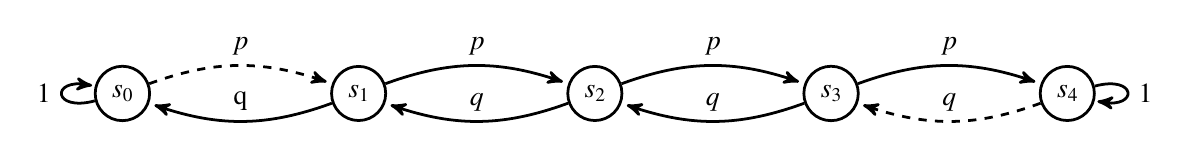
\begin{tikzpicture}[->,>=stealth',shorten >=2pt, line width=1pt, node distance=3cm] 
 \node [circle, draw] (zero) {$s_0$};
  \node [circle, draw] (one) [right of=zero] {$s_1$}; 
  \node [circle, draw] (two) [right of  = one] {$s_2$}; 
  \node [circle, draw] (three) [right of  = two] {$s_3$};
  \node [circle, draw] (four) [right of  = three] {$s_4$};
    
  \path (zero) edge [loop left] node {$1$} (zero); 
  \path [dashed, ->] (zero) edge [bend left=20]  node [above] {$p$} (one);
  
\path (one) edge  [bend left=20]  node [above] {q} (zero);
\path (one) edge [bend left=20]  node [above] {$p$} (two);

\path (two) edge [bend left = 20] node [above] {$q$} (one);
\path (two) edge [bend left=20] node [above] {$p$} (three);

\path (three) edge [bend left = 20] node [above] {$q$} (two);
\path (three) edge [bend left = 20]  node [above] {$p$} (four);

\path[dashed, ->] (four) edge [bend left = 20] node [above] {$q$} (three);
\path (four) edge [loop right] node {$1$} (four); 
 \end{tikzpicture}
	\caption{}
	\label{fig:markov}
 \end{figure}
 
 \item At time instant $n$, 
	 \begin{align}
		 \vec{p}^{\brak{n}} = \myvec{
			 P_0^{\brak{n}} \\ P_1^{\brak{n}}\\ P_2^{\brak{n}}\\ P_3^{\brak{n}} \\ P_4^{\brak{n}}}
	 \end{align}
where $P_i^{\brak{n}}$ are defined to be the {\em stationary} probabilities.

 \item
	 $P_{i|j}$ is defined as the {\em transition} probability of going to state $i$ from state $j$.
 \item For a matrix $\vec{A}$, let
 \begin{align}
 \vec{A}\vec{x} = \lambda\vec{x}.
 \end{align}
Then  $\lambda$ is a scalar defined to be the eigenvalue of $\vec{A}$ and $\vec{x}$ is the corresponding eigenvector.
\end{enumerate}

			


\subsection{Problems}
\begin{enumerate}[label=\arabic*.,ref=\thesubsection.\theenumi]
\numberwithin{equation}{enumi}
\item Let
\begin{align}
&P_0^{(n+1)} = P_0^{(n)}\\
&P_1^{(n+1)} = pP_0^{(n)} + qP_2^{(n)} \\
&P_2^{(n+1)} = pP_1^{(n)} + qP_3^{(n)} \\
&P_3^{(n+1)} = pP_2^{(n)} + qP_4^{(n)} \\
&P_4^{(n+1)} = P_4^{(n)}
\end{align}
Find the matrix $\vec{P}$ such that $\vec{p^{(n+1)}} = \vec{P}\vec{p^{(n)}}	$
\item Show that 1 is an eigen value of $\vec{P}.$
\item Show that 
\begin{align}
	P_2^{(n+1)} = pP_1^{(n)} + qP_3^{(n)}
\end{align}

\item If $P_0 =1, P_N = 0$ and
\begin{align}
P_i = p P_{i-1}+qP_{i+1}
\end{align}
	show that 
\begin{align}
P_i =	\frac{\left(\frac{p}{q}\right)^i-\left(\frac{p}{q}\right)^N}{1-\left(\frac{p}{q}\right)^N}, 0\leq i \leq N
\end{align}
%\item Find the angle between the two lines $2x = 3y = -z$ and $6x = -y = -4z$.

\end{enumerate}
\section{Gaussian Distribution}
\subsection{Definitions}
\begin{enumerate}[label=\arabic*.,ref=\thesubsection.\theenumi]
\numberwithin{equation}{enumi}
\item The CDF of $X$ is defined as,
\begin{align}
	F_X(x) = \pr{X \leq x}
\end{align}
\item The PDF of $X$ is defined as,

\begin{align}
p_X(x) = \dfrac{d}{dx}F_X(x)
\end{align}
\item Let 
 $X \sim \mathcal{N}(\mu, \sigma^2)$.  Then the 
	$Q$ function is defined as,
\begin{align}
	Q(x) = \pr{X>x}, \quad x \ge 0
\end{align}
\end{enumerate}
\subsection{Problems}
\begin{enumerate}[label=\arabic*.,ref=\thesubsection.\theenumi]
\numberwithin{equation}{enumi}
\item Find 
\begin{align}
	\pr{\abs{X-\mu} \leq k\sigma}
\end{align}
 in terms of $Q$ function.
\item Find 
\begin{align}
	\pr{X \leq x, \abs{X-\mu} \leq k\sigma}
\end{align}
		in terms of $F_X(x)$
\item Find 
\begin{align}
	F_X\brak{x | \abs{X-\mu} \leq k\sigma}
\end{align}
\item Find 
\begin{align}
	p_X\brak{x | \abs{X-\mu} \leq k\sigma}
\end{align}
\end{enumerate}
\section{Bivariate Gaussian}
\subsection{Definitions}
\begin{enumerate}[label=\arabic*.,ref=\thesubsection.\theenumi]
		\numberwithin{equation}{enumi}
\item Let
\begin{align}
	\vec{X} &= \myvec{x_1\\x_2}, \bm{\mu} = E\brak{\vec{X}}
	%\myvec{\mu_x\\\mu_y}\\
	\\
	\vec{\Sigma_{x}} &= E\sbrak{\brak{\vec{x}-\bm{\mu}}\brak{ \vec{x}-\bm{\mu}}^{\top}}
%\vec{\Sigma} = \myvec{\sigma^2_x&\rho\sigma_x\sigma_y\\\rho\sigma_x\sigma_y&\sigma^2_y}
\end{align}
		Then $\vec{\Sigma_{x}}$ is defined to be the {\em covariance} matrix  of $\vec{x}$.
\item For $\vec{x} \sim \mathcal{N}\brak{\bm{\mu}, \vec{\Sigma_{x}}}$,
\begin{align}
	f_{\vec{X}}(\vec{x}) = \frac{1}{2\pi\sqrt{\abs{\vec{\Sigma_{x}}}}}\exp{{-\frac{1}{2}\brak{\brak{\vec{x}-\bm{\mu}}^\top\vec{\Sigma_{x}}^{-1}\brak{\vec{x}-\bm{\mu}}}}}
\end{align}
\item The {\em correlation coefficient} is defined as
\begin{align}
	\rho = \frac{E\sbrak{\brak{x_1-\mu_{1}}\brak{x_2-\mu_{2}}}}{\sigma_{1}\sigma_{2}}
\end{align}
where $\mu_i,\sigma_i^2$ are the mean and variance of $x_i$.
\end{enumerate}
\subsection{Problems}
\begin{enumerate}[label=\arabic*.,ref=\thesubsection.\theenumi]
\numberwithin{equation}{enumi}
\item Show that
\begin{align}
	E\sbrak{\brak{\vec{x}-\bm{\mu}}\brak{\vec{x}-\bm{\mu}}^{\top}} = \myvec{\sigma^2_{1}&\rho\sigma_{1}\sigma_{2}\\\rho\sigma_{1}\sigma_{2}&\sigma^2_{2}}
\end{align}
\item Prove that $\vec{\Sigma_{x}}$ is a diagonal matrix when $x_1$ and $x_2$ are independent.
\item Let
\begin{align}
z_1 = x_1+x_2 \\ 
z_2 = x_1-x_2 
\end{align}
		Find $\vec{P}$ such that
\begin{align}
	\vec{z} =\myvec{z_1\\ z_2}  = \vec{P}\vec{x}
\end{align}
\item Show that 
	\begin{align} 
\vec{\Sigma_{z}} = \vec{P} \vec{\Sigma_x} \vec{P}^{\top} 
\end{align} 
\item 
	 Check the independence of $z_1$ and $z_2$ given that $\sigma_{x_1} = \sigma_{x_2}$.
\item Show that columns of $\vec{P}$ are eigenvectors of $\vec{\Sigma_z}$.
\item Show that the eigenvectors of $\vec{P}$ are orthogonal to each other.
\item Summarize your conclusion in one line.
\end{enumerate}


\end{document}
